\documentclass[letterpaper,11pt]{article}

\usepackage{amsmath}
\usepackage{amssymb}
\usepackage[hmargin=1.25in,vmargin=1in]{geometry}
\usepackage{booktabs}
\usepackage{graphicx}
\usepackage{hyperref}
\usepackage{lmodern}
\usepackage{microtype}
\usepackage{subcaption}

\title{Coursework 2: STAT 570}
\author{Philip Pham}
\date{\today}

\begin{document}
\maketitle
\begin{enumerate}
\item Consider the simple linear regression model
  \begin{equation*}
    Y_i = \beta_0 + \beta_1x_i + \epsilon_i,~i = 1,\ldots,n,
    \label{eqn:p1_model}    
  \end{equation*}
  where the error terms $\epsilon_i$ are such that
  $\mathbb{E}\left[\epsilon_i\right] = 0$,
  $\operatorname{Var}\left(\epsilon_i\right) = \sigma^2$, and
  $\operatorname{Cov}\left(\epsilon_i, \epsilon_j\right) = 0$ for $i \neq j$.

  In the following you will consider
  $x_i \sim_{\mathrm{iid}} \mathcal{N}\left(20, 3^2\right)$, with $\beta_0 = 2$
  and $\beta_1 = -2.5$ and $n=15,30$.

  Consider the model in Equation \ref{eqn:p1_model} with the error terms
  $\epsilon_i$, independent and identically distributed, from the distributions:
  \begin{itemize}
  \item The normal distribution with mean $0$ and variance $2^2$.
  \item The uniform distribution on the range $(-r,r)$ for $r = 2$.
  \item A skew normal distribution with $\alpha = 5$, $\omega = 1$, and $\xi$
    chosen to given mean $0$.
  \end{itemize}

  \begin{enumerate}
  \item What is the theoretical bias for $\hat{\beta}$ if the errors are of the
    form specified?

    \begin{description}
    \item[Solution:] The theoretical bias for $\hat{\beta}$ is $0$. Let
      \begin{equation}
        X = \begin{pmatrix}
          1 & x_1 \\
          1 & x_2 \\
          \vdots & \vdots \\
          1 & x_n
        \end{pmatrix}
        \label{eqn:p1_X}
      \end{equation}
      
      If we use the least squares estimate, we have
      \begin{align}
        \hat{\beta}
        &= \left(X^\intercal X\right)^{-1}X^\intercal y \nonumber\\
        &= \left(X^\intercal X\right)^{-1}X^\intercal\left(X\beta + \epsilon \right) \nonumber\\
        &= \beta + \left(X^\intercal X\right)^{-1}X^\intercal\epsilon,
          \label{eqn:p1_beta_hat}
      \end{align}

      Thus, using Equation \ref{eqn:p1_beta_hat} and linearity of expectations,
      we have
      \begin{equation}
        \boxed{
          \operatorname{bias}\left(\hat{\beta}\right) =
          \mathbb{E}\left[\hat{\beta}\right] - \beta =
          \beta +
          \left(X^\intercal X\right)^{-1}X^\intercal
          \mathbb{E}\left[\epsilon\right] - \beta
          = 0.
        }
        \label{eqn:p1_beta_hat_bias}
      \end{equation}
    \end{description}
  \item Compare the variance of the estimator as reported by least squares, with
    that which follows from the sampling distribution of the estimator.

    \begin{description}
    \item[Solution:] 
    \end{description}
    
  \item Examine the distribution of the resultant estimators (across
    simulations) of $\beta_0$ and $\beta_1$, in particular with respect to
    normality. For each parameter find the coverage probability of a 95\%
    confidence interval, that is the proportion of times that the confidence
    intervals contain the true value.

    \begin{description}
    \item[Solution:] 
    \end{description}
    
  \item \textbf{Bonus:} Can you ``break'' least squares? i.e., find a
    distribution of the errors (with mean zero) that produces poor confidence
    interval coverage?
    
    \begin{description}
    \item[Solution:] 
    \end{description}
  \end{enumerate}
\item Consider the exponential regression problem with independent responses
  \begin{equation}
    p\left(y_i \mid \lambda_i\right) = \lambda_i\exp\left(-\lambda_iy_i\right),
    y_i > 0,
    \label{eqn:p2_model}
  \end{equation}
  and $\log\lambda_i = \beta_0 + \beta_1x_i$ for given covariates $x_i$,
  $i = 1,\ldots,n$. We wish to estimate the $2 \times 1$ regression parameter
  $\beta = \begin{pmatrix}
    \beta_0 & \beta_1
  \end{pmatrix}^\intercal$ using maximum likelihood estimation (MLE).

  \begin{enumerate}
  \item Find expressions for the likelihood function $L\left(\beta\right)$,
    log-likelihood function $l\left(\beta\right)$, score function
    $S\left(\beta\right)$, and Fisher's information matrix $I\left(\beta\right)$.

    \begin{description}
    \item[Solution:] We can rewrite Equation \ref{eqn:p2_model} in terms of
      $\beta$, which gives us
      \begin{align}
        p\left(y_i \mid \beta_0,\beta_1\right)
        &= \exp\left(\beta_0 + \beta_1x_i\right)
        \exp\left(- y_i\exp\left(\beta_0 + \beta_1x_i\right)\right) \nonumber\\
        &=
        \exp\left(
          \beta_0 + \beta_1x_i - y_i\exp\left(\beta_0 + \beta_1x_i\right)\right)
        \label{eqn:p2_model_beta}.
      \end{align}

      Using Equation \ref{eqn:p2_model_beta}, we can write the likelihood
      function
      \begin{align}
        L\left(\beta\right)
        &= \prod_{i=1}^n p\left(y_i \mid \beta_0,\beta_1\right) \nonumber\\
        &= \exp\left(
          n\beta_0 + \beta_1\sum_{i=1}^n x_i
          -
          \sum_{i=1}^n y_i\exp\left(\beta_0 + \beta_1x_i\right)
          \right).
          \label{eqn:p2_likelihood}
      \end{align}

      Taking the log of Equation \ref{eqn:p2_likelihood}, we have the
      log-likelihood function as
      \begin{align}
        l\left(\beta\right)
        &= \log L\left(\beta\right) \nonumber\\
        &= n\beta_0 + \beta_1\sum_{i=1}^nx_i -
          \sum_{i=1}^ny_i\exp\left(\beta_0 + \beta_1x_i\right).
          \label{eqn:p2_log_likelihood}
      \end{align}

      Taking the gradient of Equation \ref{eqn:p2_log_likelihood}, we have the
      score function
      \begin{align}
        S\left(\beta\right)
        &= \nabla l\left(\beta\right) \nonumber\\
        &= \begin{pmatrix}
          n - \sum_{i=1}^ny_i\exp\left(\beta_0 + \beta_1x_i\right) \\
          \sum_{i=1}^nx_i - \sum_{i=1}^n x_iy_i\exp\left(\beta_0 + \beta_1x_i\right)
        \end{pmatrix}.
        \label{eqn:p2_score}
      \end{align}

      One definition of the Fisher information is the expected value of the
      observed information which is the negative of the second derivative of the
      log-likelihood function. For a single observation,
      \begin{align}
        \mathcal{I}_1\left(\beta\right) &= \mathbb{E}\left[          
          \begin{pmatrix}
            Y\exp\left(\beta_0 + \beta_1x_i\right)
            & x_iY\exp\left(\beta_0 + \beta_1x_i\right) \\
            x_iY\exp\left(\beta_0 + \beta_1x_i\right) &
            x_i^2Y\exp\left(\beta_0 + \beta_1x_i\right)
          \end{pmatrix} \mid X = x_i\right] \nonumber\\
        &= \frac{1}{\exp\left(\beta_0 + \beta_1x_i\right)} \begin{pmatrix}
          \exp\left(\beta_0 + \beta_1x_i\right)
          & x_i\exp\left(\beta_0 + \beta_1x_i\right) \\
          x_i\exp\left(\beta_0 + \beta_1x_i\right) &
          x_i^2\exp\left(\beta_0 + \beta_1x_i\right)
        \end{pmatrix} \nonumber\\
        &= \begin{pmatrix}
          1 & x_i \\
          x_i & x_i^2
        \end{pmatrix}
        \label{eqn:p2_fisher_information_single}      
      \end{align}
      by properties of the exponential distribution. Thus, Fisher information is
      \begin{equation}
        \mathcal{I}_n\left(\beta\right) =
        \begin{pmatrix}
          n & \sum_{i=1}^n x_i \\
          \sum_{i=1}^n x_i & \sum_{i=1}^n x_i^2
        \end{pmatrix}.
        \label{eqn:p2_fisher_information}
      \end{equation}
    \end{description}
  \item Find expressions for the maximum likelihood estimate $\hat{\beta}$. If
    no closed form solution exists, then instead provide a functional form that
    could be simply implemented for solution.

    \begin{description}
    \item[Solution:] We can solve for $\hat{\beta}_0$ in terms of
      $\hat{\beta}_1$. We know that $S\left(\hat{\beta}\right) = \mathbf{0}$.

      From Equation \ref{eqn:p2_score}, we can solve for $\hat{\beta}_0$,
      \begin{align}
        \hat{\beta}_0
        &= \log n - \log \sum_{i=1}^n y_i\exp\left(\hat{\beta}_1x_i\right).
        \label{eqn:p2_beta_0_hat}
      \end{align}

      Substituing Equation \ref{eqn:p2_beta_0_hat} into the second entry of
      Equation \ref{eqn:p2_score}, we have
      \begin{align}
        0
        &= \sum_{i=1}^n x_i -
          \exp\left(\hat{\beta}_0\right)
          \sum_{i=1}^nx_iy_i\exp\left(\hat{\beta}_1x_i\right) \nonumber\\
        &= \sum_{i=1}^n x_i -
          \frac{n}{\sum_{i=1}^ny_i\exp\left(\hat{\beta}_1x_i\right)}
          \sum_{i=1}^nx_iy_i\exp\left(\hat{\beta}_1x_i\right),
        \label{eqn:p2_beta_1_hat}
      \end{align}
      which we can solve numerically with a root-finding algorithm.            
    \end{description}
  \item For the data in Table \ref{tab:p2_data}, numerically maximize the
    likelihood function to obtain estimates of $\beta$. These data consist of
    the survival times ($y$) of rats as function of concentration of a
    contaminant ($x$). Find the asymptotic covariance matrix for your estimate
    using the information $\mathcal{I}\left(\beta\right)$. Provide a 95\%
    confidence interval for each element of $\beta_0$ and $\beta_1$.
    
    \begin{table}
      \centering
      \begin{tabular}{crr}
        \toprule
        $i$ & $x_i$ & $y_i$ \\
        \midrule
        1 & 6.1 & 0.8 \\
        2 & 4.2 & 3.5 \\
        3 & 0.5 & 12.4 \\
        4 & 8.8 & 1.1 \\
        5 & 1.5 & 8.9 \\
        6 & 9.2 & 2.4 \\
        7 & 8.5 & 0.1 \\
        8 & 8.7 & 0.4 \\
        9 & 6.7 & 3.5 \\
        10 & 6.5 & 8.3 \\
        11 & 6.3 & 2.6 \\
        12 & 6.7 & 1.5 \\
        13 & 0.2 & 16.6 \\
        14 & 8.7 & 0.1 \\
        15 & 7.5 & 1.3 \\
        \bottomrule
      \end{tabular}
      \caption{Each observation is a rat. $x_i$ are the concentrations of the
        contaminant, and $y_i$ are the survival times.}
      \label{tab:p2_data}
    \end{table}

    \begin{description}
    \item[Solution:] Numerically solving Equations \ref{eqn:p2_beta_0_hat} and
      \ref{eqn:p2_beta_1_hat}, we have that
      \begin{equation}
        \hat{\beta} =
        \begin{pmatrix}
          \hat{\beta}_0 \\
          \hat{\beta}_1
        \end{pmatrix}
        =
        \begin{pmatrix}
          -2.821150253077923 \\
          0.30133576292327585
        \end{pmatrix}.
        \label{eqn:p2_beta_hat_mle}
      \end{equation}

      The Fisher information gives a lower bound on the variance according to
      the Cram\'er-Rao bound. Asymptotic normality of the MLE tells us that
      \begin{equation*}
        \hat{\beta}_n - \beta \rightarrow
        \mathcal{N}\left(0, \mathcal{I}_n^{-1}\left(\beta\right)\right)
      \end{equation*}
      in distribution.

      Thus, we have the covariance matrix
      \begin{equation}
        \operatorname{Var}\left(\hat{\beta}\right)
        \approx \begin{pmatrix}
          15 & 90.1 \\
          90.1 & 671.07
        \end{pmatrix}^{-1}
        = \begin{pmatrix}
          0.34448471 & -0.04625162 \\
          -0.04625162 & 0.00770005
        \end{pmatrix}.
      \end{equation}

      Using this we can approximate 95\% confidence intervals as
      $\hat{\beta}_j \pm
      z_{0.975}\sqrt{\operatorname{Var}\left(\hat{\beta}_j\right)}$, where
      $z_{p} = \Phi^{-1}\left(p\right)$ and $\Phi$ is the cumulative
      distribution function of the normal distribution.

      We have the confidence intervals
      \begin{align}
        \left(
        \hat{\beta}_0 - 1.150358,
        \hat{\beta}_0 + 1.150358
        \right)
        &= \left(
          -3.97150839, -1.67079212
        \right) \nonumber\\
        \left(
        \hat{\beta}_1 - 0.171986669,
        \hat{\beta}_1 + 0.171986669
        \right)
        &= \left(
          0.12934909, 0.47332243
          \right)
          \label{eqn:p2_confidence_interval}
      \end{align}
      for $\hat{\beta}_0$ and $\hat{\beta}_1$, respectively.
      

      All calcuations can be found in
      \href{https://nbviewer.jupyter.org/github/ppham27/stat570/blob/master/hw2/exponential\_regression.ipynb}{\texttt{exponential\_regression.ipynb}}.
    \end{description}
  \item Plot the log-likelihood function $l\left(\beta_0,\beta_1\right)$ and
    compare with the log of the asymptotic normal approximation to the sampling
    distribution of the MLE.
    \label{part:2d}

    \begin{description}
    \item[Solution:] The two plots can be found in Figure
      \ref{fig:p2_beta_hat_likelihood}.

      The log-likelihood function can be found in Figure
      \ref{fig:p2_log_likelihood}, and the asymptotic normal approximation is
      plotted in Figure \ref{fig:p2_asymptotic_normal}.

      The distributions are similar, and the asymptotic normal approximation
      accurately captures the covariance structure of $\hat{\beta}$.  The
      asymptotic normal approximation, however, does underestimate the
      variance. This is unsurprising since the inverse of the Fisher information
      matrix is a lower bound on variance according to the Cram\'er-Rao bound.

      Code for the plots can be found in
      \href{https://nbviewer.jupyter.org/github/ppham27/stat570/blob/master/hw2/exponential\_regression.ipynb}{\texttt{exponential\_regression.ipynb}}.
      
      \begin{figure}
        \begin{subfigure}[b]{\textwidth}
          \centering
          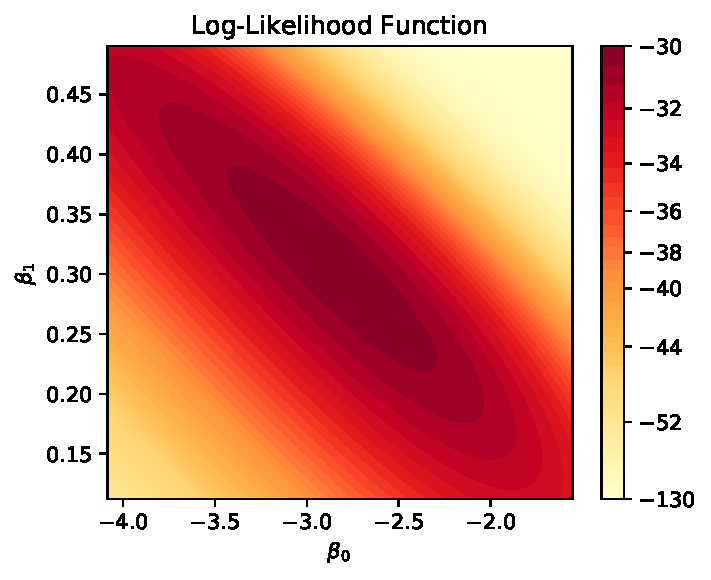
\includegraphics{p2_log_likelihood.pdf}
          \caption{The log-likelihood function is centered at the MLE estimate.}
          \label{fig:p2_log_likelihood}
        \end{subfigure}
        \begin{subfigure}[b]{\textwidth}
          \centering
          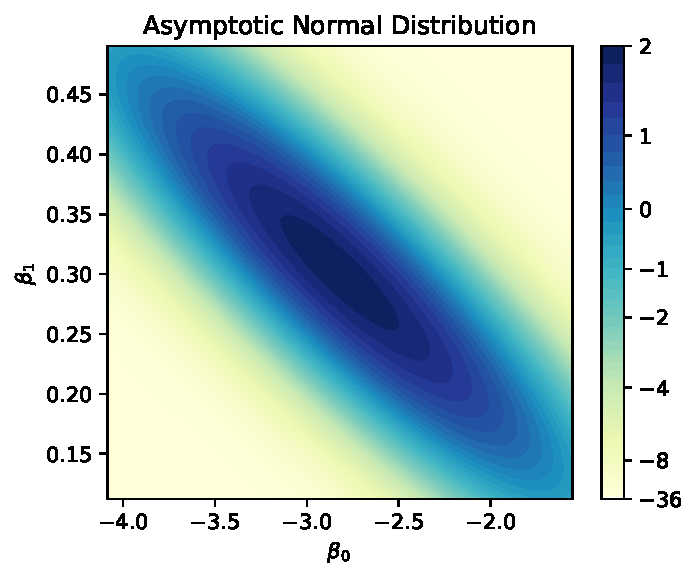
\includegraphics{p2_asymptotic_normal.pdf}
          \caption{The asymptotic normal approximation mirrors the
            log-likelihood with slightly less variance.}
          \label{fig:p2_asymptotic_normal}
        \end{subfigure}
        \caption{Plots of the distributions of $\hat{\beta}$ for Part
          \ref{part:2d}.}
        \label{fig:p2_beta_hat_likelihood}
      \end{figure}      
    \end{description}
    
  \item Summarize the results of the estimation presented above in a manner that
    would address the question of whether increasing concentrations of the
    contaminant had an effect on a rat's life expectancy.

    \begin{description}
    \item[Solution:] $\lambda_i$ can be viewed as the rate of death, so the mean
      survival time is $\lambda_i^{-1}$. $\log\lambda_i$ has a linear
      relationship with concentrations of the contaminant described by
      $\beta_1$. $\beta_1 > 0$ indicates that increasing concentrations of the
      contaminant increase death rates, and therefore, decrease life expectancy.

      Indeed from Equation \ref{eqn:p2_beta_hat_mle}, our estimate of $\beta_1$,
      $\hat{\beta}_1 = 0.30133576292327585 > 0$. From Equation
      \ref{eqn:p2_confidence_interval}, we see that the 95\% confidence interval
      lies entirely on the positive half-line, so the result is statistically
      significant at level $0.05$.

      Thus, it is quite likely that increasing concentrations of the contaminant
      decrease life expectancy.
    \end{description}
  \end{enumerate}  
\end{enumerate}

\end{document}
